\documentclass{article}

% Font
\usepackage{mlmodern}

% Margins
\usepackage[margin=1in]{geometry}

% Math symbols, proof environments
\usepackage{amsmath, amsthm, amssymb}

% Use this package for matrices
\usepackage{array}

% Images and positioning
\usepackage{graphicx, float, tikz}

% Trees
\usepackage{forest}

% Plots
\usepackage{pgfplots}

\usepackage{xcolor}

\usepackage{parskip}
\usepackage[T1]{fontenc}

% Math commands
\newcommand{\R}{\mathbb{R}} % Real numbers
\newcommand{\Z}{\mathbb{Z}} % Integers
\newcommand{\C}{\mathbb{C}} % Complex numbers
\newcommand{\Pw}{\mathcal{P}}
\newcommand{\set}[1]{\left\{ #1 \right\}}
\newcommand{\setc}[2]{\left\{ #1 \middle| #2 \right\}}
\newcommand{\abs}[1]{\left| #1 \right|}
\newcommand{\var}{\mathrm{VAR}}
\newcommand{\ut}[1]{\text{ #1}}
\newcommand{\cov}{\mathrm{COV}}
\newcommand{\intR}{\int_{-\infty}^{\infty}}
\newcommand{\red}[1]{\textcolor{red}{#1}}
\newcommand{\blu}[1]{\textcolor{blue}{#1}}
\newcommand{\grn}[1]{\textcolor{green}{#1}}
\newcommand{\contradiction}{\Rightarrow\!\Leftarrow}
\newcommand{\fun}{\mathrm{Fun}}

\DeclareMathOperator{\pMat}{Mat}
\newcommand{\Mat}[2]{\pMat_{#1 \times #2}}
\DeclareMathOperator{\spn}{span}
\DeclareMathOperator{\Ker}{Ker}
\DeclareMathOperator{\Img}{Im}
\DeclareMathOperator{\rank}{rank}
\DeclareMathOperator{\nul}{null}
\DeclareMathOperator{\tr}{tr}
\newcommand{\angles}[1]{\left \langle #1 \right \rangle}
\newcommand{\conj}[1]{\overline{#1}}

\title{Math 168 Homework 1}

\author{Jason Cheng}

\date{\today}

\begin{document}

\maketitle

\subsection*{Exercise 1}

Dr. Körner thinks that students should treat lectures as a dialogue where the
student is following the arguments rather than blindly take notes.

\newpage

\subsection*{Exercise 2}

\newpage

\subsection*{Exercise 3}

\begin{enumerate}
  \item[1.]
  A polygon is a static simple network. The nodes are the vertices and the edges
  are the sides of the polygon.
  
  \item[2.]
  Family trees are dynamic (because relationships can form/change) bipartite
  (because it's a tree) networks. The nodes are the family members and the edges
  are the relationships between parents and children.

  \item[3.]
  Rivers are observable transport networks. The nodes are lakes and oceans, and
  the edges are rivers.

  \item[4.]
  Plumbing is a weighted (weighted by pipe thickness) network with directed
  edges. The nodes are faucets, and the edges are the pipes.
\end{enumerate}

\newpage

\subsection*{Exercise 4}

\begin{enumerate}
  \item[(a)]
  \begin{gather*}
    A =
    \begin{bmatrix}
      0 & 1 & 1 & 1 \\
      1 & 0 & 1 & 1 \\
      1 & 1 & 0 & 1 \\
      1 & 1 & 1 & 0
    \end{bmatrix} \\
    L = A - D =
    = \boxed{
      \begin{bmatrix}
        -3 & 1 & 1 & 1 \\
        1 & -3 & 1 & 1 \\
        1 & 1 & -3 & 1 \\
        1 & 1 & 1 & -3
      \end{bmatrix}
    }
  \end{gather*}

  \item[(b)]
  There would be \( \binom{|N|}{2} \) edges.

  \item[(c)]
  \begin{align*}
    \det(A - \lambda I) &= \det
    \begin{pmatrix}
      -\lambda & 1 & 1 & 1 \\
      1 & -\lambda & 1 & 1 \\
      1 & 1 & -\lambda & 1 \\
      1 & 1 & 1 & -\lambda \\
    \end{pmatrix} \\
    &= \lambda^4 - 6\lambda^2 - 8\lambda - 3 \\
    &= \lambda^4 - 2\lambda^2 + 1 - 4\lambda^2 - 8\lambda - 4 \\
    &= (\lambda^2 - 1)^2 - 4(\lambda + 1)^2 \\
    &= (\lambda - 1)^2 (\lambda + 1)^2 - 4(\lambda + 1)^2 \\
    &= (\lambda + 1)^2 ((\lambda - 1)^2 - 4) \\
    &= (\lambda + 1)^3 (\lambda - 3) \\
  \end{align*}

  The eigenvalues of \( A \) are \( \lambda = -1, 3 \). \( \lambda = -1 \) has
  algebraic multiplicity of 3.

  \item[(d)]
  \begin{align*}
    \det(L - \lambda I) &= \det
    \begin{pmatrix}
      -3 - \lambda & 1 & 1 & 1 \\
      1 & -3 - \lambda & 1 & 1 \\
      1 & 1 & -3 - \lambda & 1 \\
      1 & 1 & 1 & -3 - \lambda
    \end{pmatrix} \\
    &= \lambda^4 + 12\lambda^3 + 48\lambda^2 + 64\lambda \\
    &= \lambda^4 + 8\lambda^3 + 16\lambda^2 + 4\lambda^3 + 32\lambda^2 + 64\lambda \\
    &= \lambda^2 (\lambda + 4)^2 + 4\lambda (\lambda + 4)^2 \\
    &= \lambda (\lambda + 4)^3
  \end{align*}

  The eigenvalues of \( L \) are \( \lambda = -4, 0 \).
\end{enumerate}

\newpage

\subsection*{Exercise 5}

\begin{enumerate}
  \item[(a)]
  Adjacency matrix:
  \[
    A =
    \begin{bmatrix}
      0 & 1 & 1 \\
      1 & 0 & 1 \\
      1 & 1 & 0
    \end{bmatrix}
  \]

  \begin{align*}
    A^2 &=
    \begin{bmatrix}
      0 & 1 & 1 \\
      1 & 0 & 1 \\
      1 & 1 & 0
    \end{bmatrix}
    \begin{bmatrix}
      0 & 1 & 1 \\
      1 & 0 & 1 \\
      1 & 1 & 0
    \end{bmatrix} \\
    &=
    \begin{bmatrix}
      2 & 1 & 1 \\
      1 & 2 & 1 \\
      1 & 1 & 2
    \end{bmatrix} \\
    A^3 &=
    \begin{bmatrix}
      2 & 1 & 1 \\
      1 & 2 & 1 \\
      1 & 1 & 2
    \end{bmatrix}
    \begin{bmatrix}
      0 & 1 & 1 \\
      1 & 0 & 1 \\
      1 & 1 & 0
    \end{bmatrix} \\
    &=
    \begin{bmatrix}
      2 & 3 & 3 \\
      3 & 2 & 3 \\
      3 & 3 & 2
    \end{bmatrix}
  \end{align*}

  \( A^3_{11} = 2 \), so there are two paths of length 3 that start and end at
  node 1.

  \item[(b)]
  The entries of \( A^3 \) outside the main diagonal are all 3, so between each
  pair of different nodes there are 3 paths.
\end{enumerate}

\newpage

\subsection*{Exercise 6}

Adjacency matrix:
\[
  A =
  \begin{bmatrix}
    0 & 1 & 1 & \dotso \\
    1 & 0 & 0 & \dotso \\
    1 & 0 & 0 & \dotso \\
    \vdots & \vdots & \vdots & \ddots \\
  \end{bmatrix}_{n \times n}
\]

\begin{align*}
  &\det(A - \lambda I) \\
  &= \det
  \begin{pmatrix}
    -\lambda & 1 & 1 & \dotso \\
    1 & -\lambda & 0 & \dotso \\
    1 & 0 & -\lambda & \dotso \\
    \vdots & \vdots & \vdots & \ddots
  \end{pmatrix}_{n \times n} \\
  &= -1 \cdot \det
  \begin{pmatrix}
    1 & 1 & 1 & \dotso \\
    0 & -\lambda & 0 & \dotso \\
    0 & 0 & -\lambda & \dotso \\
    \vdots & \vdots & \vdots & \ddots
  \end{pmatrix}_{(n - 1) \times (n - 1)}
  - \lambda \det
  \begin{pmatrix}
    -\lambda & 1 & 1 & \dotso \\
    1 & -\lambda & 0 & \dotso \\
    1 & 0 & -\lambda & \dotso \\
    \vdots & \vdots & \vdots & \ddots
  \end{pmatrix}_{(n - 1) \times (n - 1)} \\
\end{align*}
\begin{align*}
  &\det
  \begin{pmatrix}
    1 & 1 & 1 & \dotso \\
    0 & -\lambda & 0 & \dotso \\
    0 & 0 & -\lambda & \dotso \\
    \vdots & \vdots & \vdots & \ddots
  \end{pmatrix}_{n \times n} \\
  &= -\lambda \det
  \begin{pmatrix}
    1 & 1 & 1 & \dotso \\
    0 & -\lambda & 0 & \dotso \\
    0 & 0 & -\lambda & \dotso \\
    \vdots & \vdots & \vdots & \ddots
  \end{pmatrix}_{(n - 1) \times (n - 1)}
\end{align*}
\begin{align*}
  f(n) &= -g(n - 1) - \lambda f(n - 1) \\
  g(n) &= -\lambda g(n - 1) \\
  g(2) &= \det
  \begin{pmatrix}
    1 & 1 \\
    0 & -\lambda 
  \end{pmatrix} \\
  &= -\lambda \\
  g(n) &= (-\lambda)^{n - 1} \\
  f(2) &= \det
  \begin{pmatrix}
    -\lambda & 1 \\
    1 & -\lambda
  \end{pmatrix} \\
  &= \lambda^2 - 1 \\
  f(n) &= (-\lambda)^n - (n - 1) (-\lambda)^{n - 2} \\
\end{align*}

Verify \( f(n) \). Base case:
\[ f(2) = (-\lambda)^2 - (2 - 1) (-\lambda)^{0} = \lambda^2 - 1 \]
Inductive step:
\begin{align*}
  f(n + 1) &= -g(n) - \lambda f(n) \\
  &= -(-\lambda)^{n - 1} - \lambda ((-\lambda)^n - (n - 1) (-\lambda)^{n - 2}) \\
  &= -(-\lambda)^{n - 1} + (-\lambda)^{n + 1} - (n - 1) (-\lambda)^{n - 1} \\
  &= (-\lambda)^{n + 1} - n (-\lambda)^{n - 1}
\end{align*}

The characteristic polynomial is \( f(n) = (-\lambda)^n - (n - 1) (-\lambda)^{n - 2} = (-\lambda)^{n - 2} ((-\lambda)^2 - (n - 1)) \).

The roots are \( \lambda = 0, \lambda = \pm \sqrt{n - 1} \).

The largest eigenvalue is \( \boxed{\sqrt{n - 1}} \).

\newpage

\subsection*{Exercise 7}

\begin{enumerate}
  \item[(a)]
  Eigenvalues:
  \begin{verbatim}
3.749429478214337+0i
-2.3540236479908256+0i
-1.5423248829430551+0i
0.14691905271954572+0i
0.000000000000000021895643135715098+0i
  \end{verbatim}

  \item[(b)]
  Graph of the network:

  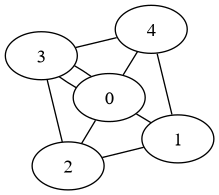
\includegraphics{ex7.png}
\end{enumerate}

\newpage

\subsection*{Exercise 8}

\end{document}
